%package list
\documentclass{article}
\usepackage[top=3cm, bottom=3cm, outer=3cm, inner=3cm]{geometry}
\usepackage{multicol}
\usepackage{graphicx}
\usepackage{url}
%\usepackage{cite}
\usepackage{hyperref}
\usepackage{array}
%\usepackage{multicol}
\newcolumntype{x}[1]{>{\centering\arraybackslash\hspace{0pt}}p{#1}}
\usepackage{natbib}
\usepackage{pdfpages}
\usepackage{multirow}
\usepackage[normalem]{ulem}
\useunder{\uline}{\ul}{}
\usepackage{svg}
\usepackage{xcolor}
\usepackage{listings}
\lstdefinestyle{ascii-tree}{
    literate={├}{|}1 {─}{--}1 {└}{+}1 
  }
\lstset{basicstyle=\ttfamily,
  showstringspaces=false,
  commentstyle=\color{red},
  keywordstyle=\color{blue}
}
%\usepackage{booktabs}
\usepackage{caption}
\usepackage{subcaption}
\usepackage{float}
\usepackage{array}

\newcolumntype{M}[1]{>{\centering\arraybackslash}m{#1}}
\newcolumntype{N}{@{}m{0pt}@{}}


%%%%%%%%%%%%%%%%%%%%%%%%%%%%%%%%%%%%%%%%%%%%%%%%%%%%%%%%%%%%%%%%%%%%%%%%%%%%
%%%%%%%%%%%%%%%%%%%%%%%%%%%%%%%%%%%%%%%%%%%%%%%%%%%%%%%%%%%%%%%%%%%%%%%%%%%%
\newcommand{\itemEmail}{schirinosne@unsa.edu.pe / rvizac@unsa.edu.pe}
\newcommand{\itemStudent}{Sebastian Arley Chirinos Negrón  /Rodrigo Estefano Viza Cuti}
\newcommand{\itemCourse}{Estructura de datos y Algoritmos}
\newcommand{\itemCourseCode}{1702124}
\newcommand{\itemSemester}{I}
\newcommand{\itemUniversity}{Universidad Nacional de San Agustín de Arequipa}
\newcommand{\itemFaculty}{Facultad de Ingeniería de Producción y Servicios}
\newcommand{\itemDepartment}{Departamento Académico de Ingeniería de Sistemas e Informática}
\newcommand{\itemSchool}{Escuela Profesional de Ingeniería de Sistemas}
\newcommand{\itemAcademic}{2023 - A}
\newcommand{\itemInput}{24 Julio 2023}
\newcommand{\itemOutput}{31 Julio 2023}
\newcommand{\itemPracticeNumber}{08}
\newcommand{\itemTheme}{Compresión}
%%%%%%%%%%%%%%%%%%%%%%%%%%%%%%%%%%%%%%%%%%%%%%%%%%%%%%%%%%%%%%%%%%%%%%%%%%%%
%%%%%%%%%%%%%%%%%%%%%%%%%%%%%%%%%%%%%%%%%%%%%%%%%%%%%%%%%%%%%%%%%%%%%%%%%%%%

\usepackage[english,spanish]{babel}
\usepackage[utf8]{inputenc}
\AtBeginDocument{\selectlanguage{spanish}}
\renewcommand{\figurename}{Figura}
\renewcommand{\refname}{Referencias}
\renewcommand{\tablename}{Tabla} %esto no funciona cuando se usa babel
\AtBeginDocument{%
	\renewcommand\tablename{Tabla}
}

\usepackage{fancyhdr}
\pagestyle{fancy}
\fancyhf{}
\setlength{\headheight}{30pt}
\renewcommand{\headrulewidth}{1pt}
\renewcommand{\footrulewidth}{1pt}
\fancyhead[L]{\raisebox{-0.2\height}{
\includegraphics[width=3cm]{img/logo_episunsa.png}}}
\fancyhead[C]{\fontsize{7}{7}\selectfont	\itemUniversity \\ \itemFaculty \\ \itemDepartment \\ \itemSchool \\ \textbf{\itemCourse}}
\fancyhead[R]{\raisebox{-0.2\height}{
\includegraphics[width=1.2cm]{img/logo_abet}}}
\fancyfoot[L]{Sebastian C./ Rodrivo V.}
\fancyfoot[C]{\itemCourse}
\fancyfoot[R]{Página \thepage}

% para el codigo fuente
\usepackage{listings}
\usepackage{color, colortbl}
\definecolor{dkgreen}{rgb}{0,0.6,0}
\definecolor{gray}{rgb}{0.5,0.5,0.5}
\definecolor{mauve}{rgb}{0.58,0,0.82}
\definecolor{codebackground}{RGB}{255, 230, 180}
\definecolor{tablebackground}{rgb}{0.8, 0, 0}

\lstset{frame=tb,
	language=bash,
	aboveskip=3mm,
	belowskip=3mm,
	showstringspaces=false,
	columns=flexible,
	basicstyle={\small\ttfamily},
	numbers=none,
	numberstyle=\tiny\color{gray},
	keywordstyle=\color{blue},
	commentstyle=\color{dkgreen},
	stringstyle=\color{mauve},
	breaklines=true,
	breakatwhitespace=true,
	tabsize=3,
	backgroundcolor= \color{codebackground},
}

\begin{document}
	
	\vspace*{10px}
	
	\begin{center}	
		\fontsize{17}{17} \textbf{ Informe de Laboratorio \itemPracticeNumber}
	\end{center}
	\centerline{\textbf{\Large Tema: \itemTheme}}
	%\vspace*{0.5cm}	

	\begin{flushright}
		\begin{tabular}{|M{2.5cm}|N|}
			\hline 
			\rowcolor{tablebackground}
			\color{white} \textbf{Nota}  \\
			\hline 
			     \\[30pt]
			\hline 			
		\end{tabular}
	\end{flushright}	

	\begin{table}[H]
		\begin{tabular}{|x{4.7cm}|x{4.8cm}|x{4.8cm}|}
			\hline 
			\rowcolor{tablebackground}
			\color{white} \textbf{Estudiante} & \color{white}\textbf{Escuela}  & \color{white}\textbf{Asignatura}   \\
			\hline 
			{\itemStudent \par \itemEmail} & \itemSchool & {\itemCourse \par Semestre: \itemSemester \par Código: \itemCourseCode}     \\
			\hline 			
		\end{tabular}
	\end{table}		
	
	\begin{table}[H]
		\begin{tabular}{|x{4.7cm}|x{4.8cm}|x{4.8cm}|}
			\hline 
			\rowcolor{tablebackground}
			\color{white}\textbf{Laboratorio} & \color{white}\textbf{Tema}  & \color{white}\textbf{Duración}   \\
			\hline 
			\itemPracticeNumber & \itemTheme & 04 horas   \\
			\hline 
		\end{tabular}
	\end{table}
	
	\begin{table}[H]
		\begin{tabular}{|x{4.7cm}|x{4.8cm}|x{4.8cm}|}
			\hline 
			\rowcolor{tablebackground}
			\color{white}\textbf{Semestre académico} & \color{white}\textbf{Fecha de inicio}  & \color{white}\textbf{Fecha de entrega}   \\
			\hline 
			\itemAcademic & \itemInput &  \itemOutput  \\
			\hline 
		\end{tabular}
	\end{table}
	
	\section{Tarea}
	\subsection{Compresión}
	\begin{itemize}
		
		\item La compresión de texto con el algoritmo de Huffman es una técnica utilizada para reducir el tamaño de archivos de texto al codificarlos de manera eficiente. Este algoritmo fue propuesto por David A. Huffman en 1952 y se basa en la idea de asignar códigos más cortos a los caracteres que aparecen con mayor frecuencia en el texto y códigos más largos a los caracteres menos frecuentes.

		\item El proceso de compresión con el algoritmo de Huffman implica los siguientes pasos:
		
		1. Análisis de frecuencias: Se analiza el texto para determinar la frecuencia de aparición de cada caracter. Los caracteres más frecuentes recibirán códigos más cortos, y los menos frecuentes recibirán códigos más largos.
		
		2. Construcción del árbol de Huffman: Se crea un árbol binario donde los nodos hoja representan los caracteres y los nodos internos son la suma de las frecuencias de sus nodos hijos. Este árbol se construye de manera que los caracteres más frecuentes estén más cerca de la raíz y los menos frecuentes estén en las hojas más alejadas.
		
		3. Asignación de códigos: Recorriendo el árbol de Huffman, se asignan códigos binarios a cada caracter, tomando un camino a la izquierda cuando se encuentra un "0" y un camino a la derecha cuando se encuentra un "1".
		
		4. Codificación del texto: Finalmente, el texto original se reemplaza por su representación en forma de secuencia de códigos binarios, utilizando la asignación de códigos realizada en el paso anterior.
		
		\item La compresión con el algoritmo de Huffman es eficiente para reducir el tamaño de archivos de texto, especialmente cuando hay caracteres que aparecen con mucha frecuencia.
		 Los caracteres más comunes tendrán códigos cortos, lo que ayuda a lograr una mayor compresión en comparación con codificaciones fijas donde todos los caracteres tienen la misma longitud de código.
		
		\item Al ser un algoritmo sin pérdida, la compresión con Huffman permite recuperar el texto original sin ninguna pérdida de información. La descompresión implica recorrer el árbol de Huffman utilizando la secuencia de códigos binarios y reemplazando los códigos con los caracteres correspondientes hasta que se obtiene el texto original.
		
		\item Es importante tener en cuenta que la compresión con el algoritmo de Huffman es más efectiva en textos largos con patrones repetitivos o caracteres que se repiten con frecuencia. En textos muy cortos o con una distribución de caracteres uniforme, la compresión puede no ser significativa o incluso puede aumentar el tamaño del archivo.
		
		\item La compresión de texto con el algoritmo de Huffman es ampliamente utilizado en aplicaciones donde el espacio de almacenamiento o el ancho de banda son limitados, como en la compresión de archivos, transmisión de datos en redes, y otras aplicaciones donde se requiere una reducción del tamaño del texto sin perder información.

	\end{itemize}	
		

	\section{URL de Repositorio Github}
	\begin{itemize}
		\item URL del Repositorio GitHub para clonar o recuperar.
		\item \url{https://github.com/Dan-Ar5/eda-lab-b-23a-b}
	\end{itemize}
	
	\section{Ejercicios designados}

	\subsection{Clase Nodo}
	\lstinputlisting[language=Java, caption={NodoHuff.java},numbers=left,]{src/NodoHuff.java}	
	\begin{itemize}
		
\item Línea 1-5: Se define la clase `NodoHuff` que implementa la interfaz `Comparable<NodoHuff>`. La clase tiene los siguientes atributos y métodos:
   - `private final int frequency;`: Atributo privado y final que almacena la frecuencia (cantidad de apariciones) del nodo.
   - `private int height = 1;`: Atributo privado que representa la altura del nodo en el árbol de Huffman, inicializado en 1.
   - `public void setData(String data) { this.data = data; }`: Método público que establece el contenido del nodo a partir de un dato de tipo `String`.
   - `private String data = "";`: Atributo privado que almacena el contenido del nodo. Se inicializa como una cadena vacía.
   - `private NodoHuff left;`: Atributo privado de tipo `NodoHuff` que representa el hijo izquierdo del nodo.
   - `private NodoHuff right;`: Atributo privado de tipo `NodoHuff` que representa el hijo derecho del nodo.

\item Línea 7-11: Se define el constructor de la clase `NodoHuff` que recibe un parámetro `freq` de tipo `int`. Este constructor se utiliza para crear un nodo hoja con la frecuencia especificada. La frecuencia se almacena en el atributo `frequency`.

\item Línea 12-20: Se define otro constructor de la clase `NodoHuff` que recibe dos parámetros `left` y `right`, ambos de tipo `NodoHuff`. Este constructor se utiliza para crear un nodo interno que tiene dos hijos. Calcula su frecuencia como la suma de las frecuencias de sus hijos y la almacena en el atributo `frequency`. El contenido del nodo se establece como la representación en cadena de la frecuencia.

\item Línea 22-26: Se define el método público `getHeight()` que devuelve la altura del nodo en el árbol de Huffman.

\item Línea 27-31: Se define el método público `setHeight()` que permite establecer la altura del nodo en el árbol de Huffman.

\item Línea 33-37: Se define el método público `getData()` que devuelve el contenido del nodo (carácter o frecuencia).

\item Línea 39-43: Se define el método público `getRight()` que devuelve el hijo derecho del nodo.

\item Línea 45-49: Se define el método público `getLeft()` que devuelve el hijo izquierdo del nodo.

\item Línea 52-58: Se sobrescribe el método `compareTo()` de la interfaz `Comparable`. Este método se utiliza para comparar dos nodos en función de su frecuencia. Devuelve un valor negativo si la frecuencia del nodo actual es menor, cero si son iguales, y un valor positivo si es mayor.

\item Línea 60-64: Se define el método público `getFrecuency()` que devuelve la frecuencia del nodo.

\item Línea 66-70: Se define el método público `getFrequency()` que devuelve la frecuencia del nodo. Este método es exactamente igual al anterior `getFrecuency()`.	\end{itemize}
	
	%%%%%%%%%%%%%%%%%%%%%%%%%%%%%%%%%%%%%%%%%%%%%%%%%%%%%%%%%%%%%%%%%%%%%%%%%%%%%%%%%%%%%%%%%%%%%
	\subsection{Clase Hoja}
	
	\lstinputlisting[language=Java, caption={Leaf.java},numbers=left,]{src/Leaf.java}	
	\begin{itemize}	
		\item Línea 1-6: Se define la clase `Leaf`, que extiende de la clase `NodoHuff`, lo que significa que `Leaf` es una subclase de `NodoHuff`. Esto indica que `Leaf` hereda todos los atributos y métodos de la clase `NodoHuff`.

\item Línea 8-10: Se declara un atributo `caracter` de tipo `char`, que representa el carácter almacenado en este nodo hoja.

\item Línea 12-14: Se declara un atributo `data` de tipo `String`, que almacenará una representación de la frecuencia y el carácter en este nodo hoja.

\item Línea 16-18: Se define un método `getCaracter()` que devuelve el carácter almacenado en este nodo hoja.

\item Línea 20-27: Se define el constructor de la clase `Leaf`, que recibe como parámetros un carácter `caracter` y una frecuencia `freq`. El constructor utiliza `super(freq)` para llamar al constructor de la clase padre `NodoHuff` y asignar la frecuencia al nodo hoja. Luego, se asigna el carácter y se construye la cadena `data` que contiene el carácter y su frecuencia.

\item Línea 29-31: Se define el método `getData()`, que devuelve la cadena `data` que contiene el carácter y su frecuencia.


	\end{itemize}	

%%%%%%%%%%%%%%%%%%%%%%%%%%%%%%%%%%%%%%%%%%%%%%%%%%%%%%%%%%%%%%%%%%%%%%%%%%%%%%%%%%%%%%%%%%%%%%%%%%%%%%%%%%
\subsection{Clase HuffmanTree.java}

\lstinputlisting[language=Java, caption={HuffmanTree.java},numbers=left,]{src/HuffmanTree.java}	
\begin{itemize}
	\item Línea 1-7: Se importan las clases necesarias para el funcionamiento del programa.

\item Línea 9-23: Se define la clase `HuffmanTree`, que representa el árbol de Huffman. Esta clase contiene varios atributos, incluyendo el nodo raíz del árbol (`root`), el texto que se desea comprimir (`text`), un mapa que almacena la frecuencia de cada carácter en el texto (`charFreq`), y un mapa que almacena los códigos Huffman de cada carácter (`huffmanCod`). El constructor de la clase recibe el texto que se desea comprimir y llama al método `fillCharFreqMap()` para calcular las frecuencias de los caracteres en el texto.

\item Línea 25-35: Se define el método `fillCharFreqMap()`, que calcula la frecuencia de cada carácter en el texto y los almacena en el mapa `charFreq`.

\item Línea 37-41: Se define el método `getRoot()`, que devuelve el nodo raíz del árbol de Huffman.

\item Línea 43-63: Se define el método `encode()`, que realiza la codificación del texto utilizando el algoritmo de Huffman. Primero, se crea una cola de prioridad (`cola`) que contiene nodos hoja para cada carácter y su frecuencia. Luego, se utiliza la cola de prioridad para construir el árbol de Huffman y se generan los códigos Huffman para cada carácter. Finalmente, se devuelve el texto codificado.

\item Línea 65-82: Se define el método `generateHuffmanCodes()`, que genera los códigos Huffman para cada carácter en el árbol. Este método es recursivo y utiliza un código binario (`code`) para representar el camino hacia cada nodo hoja. Los códigos Huffman se almacenan en el mapa `huffmanCod`.

\item Línea 84-92: Se define el método `getEncodeText()`, que devuelve el texto codificado a partir de los códigos Huffman generados para cada carácter en el texto original.

\item Línea 94-119: Se define el método `decode()`, que realiza la decodificación del texto codificado utilizando el árbol de Huffman. El método recibe el texto codificado y utiliza el árbol para seguir el camino de cada bit (`0` o `1`) y obtener el carácter original. El texto decodificado se almacena en un `StringBuilder` y se devuelve al final del método.

\item Línea 121-135: Se definen los métodos `updateHeight()` y `height()`, que se utilizan para actualizar y obtener la altura de un nodo en el árbol de Huffman, respectivamente.

\item Línea 137-147: Se define el método `printCodes()`, que imprime los caracteres junto con sus respectivos códigos Huffman en la consola.

En resumen, el código implementa el algoritmo de compresión de Huffman para codificar y decodificar textos utilizando un árbol de Huffman. El árbol de Huffman se construye a partir de las frecuencias de los caracteres en el texto y se utiliza para generar los códigos Huffman para cada carácter. La codificación y decodificación del texto se realizan siguiendo el camino de cada carácter en el árbol de Huffman.
\end{itemize}

%%%%%%%%%%%%%%%%%%%%%%%%%%%%%%%%%%%%%%%%%%%%%%%%%%%%%%%%%%%%%%%%%%%%%%%%%%%%%%%%%%%%%%%%%%%%%%%%%%
\subsection{APP TextCompressor.java}
	
\lstinputlisting[language=Java, caption={TextCompressor.java},numbers=left,]{src/TextCompressor.java}	
\begin{itemize}
	\item Línea 1-18: Se importan las clases necesarias para el funcionamiento del programa, incluyendo las relacionadas con la interfaz gráfica (swing) y las de GraphStream para visualizar el árbol de Huffman.

\item Línea 20-24: Se define la clase `TextCompressor`, que extiende la clase `javax.swing.JFrame` para crear una ventana de interfaz gráfica para la compresión y descompresión de texto. El constructor de la clase inicializa la interfaz y establece el título de la ventana.

\item Línea 27-271: Se define el código generado automáticamente para inicializar la interfaz gráfica. Este código crea los componentes visuales, como botones, áreas de texto y etiquetas, y los posiciona en la ventana.

\item Línea 38-59: Se definen los métodos `btDecodeMouseClicked()` y `btEncodeMouseClicked()`, que se ejecutan cuando se hace clic en los botones "DESCOMPRIMIR" y "COMPRIMIR" respectivamente. Estos métodos se encargan de realizar la compresión y descompresión del texto utilizando la clase `HuffmanTree`. También se crea un grafo para visualizar el árbol de Huffman utilizando GraphStream.

\item Línea 65-70: Se define el método `main()`, que es el punto de entrada del programa. En este método se crea una instancia de la clase `TextCompressor` y se muestra la ventana de la interfaz gráfica.

\item Línea 73-128: Se define el método `crearGrafo()`, que crea y muestra un grafo utilizando GraphStream para visualizar el árbol de Huffman. El método recibe el texto que se va a comprimir, crea una instancia de la clase `HuffmanTree`, y utiliza los métodos de esta clase para generar el árbol de Huffman y codificar el texto. Luego, crea el grafo y agrega los nodos y aristas correspondientes a cada nodo del árbol de Huffman.

\item Línea 130-166: Se define el método `addNodesToGraph()`, que es un método recursivo utilizado por `crearGrafo()` para agregar los nodos y aristas al grafo. Este método recibe el nodo actual del árbol de Huffman (`current`), el grafo en el que se agregarán los nodos y aristas (`graph`), y las coordenadas (`x` e `y`) para la posición del nodo en la visualización del grafo. El método agrega el nodo actual al grafo y luego agrega los nodos hijos recursivamente, conectándolos con aristas etiquetadas con "0" y "1" para indicar el camino hacia cada hijo.

\item Línea 169-182: Se define una hoja de estilo (`styleSheet`) para la representación visual de los nodos y aristas en el grafo de Huffman. Especifica el tamaño y el color de los nodos, así como el tamaño y el color de las etiquetas de las aristas.

En resumen, el código implementa una interfaz gráfica (`TextCompressor`) para comprimir y descomprimir texto utilizando el algoritmo de Huffman. La interfaz muestra campos de texto para ingresar el texto a comprimir y mostrar el texto comprimido y descomprimido. También hay botones para realizar las operaciones de compresión y descompresión. Además, utiliza la biblioteca GraphStream para visualizar el árbol de Huffman generado durante el proceso de compresión y descompresión.
\end{itemize}
\subsection{Ejecución}
\begin{itemize}	
	\item EJECUCION 1
\end{itemize}	
\begin{figure}[H]
	\centering
	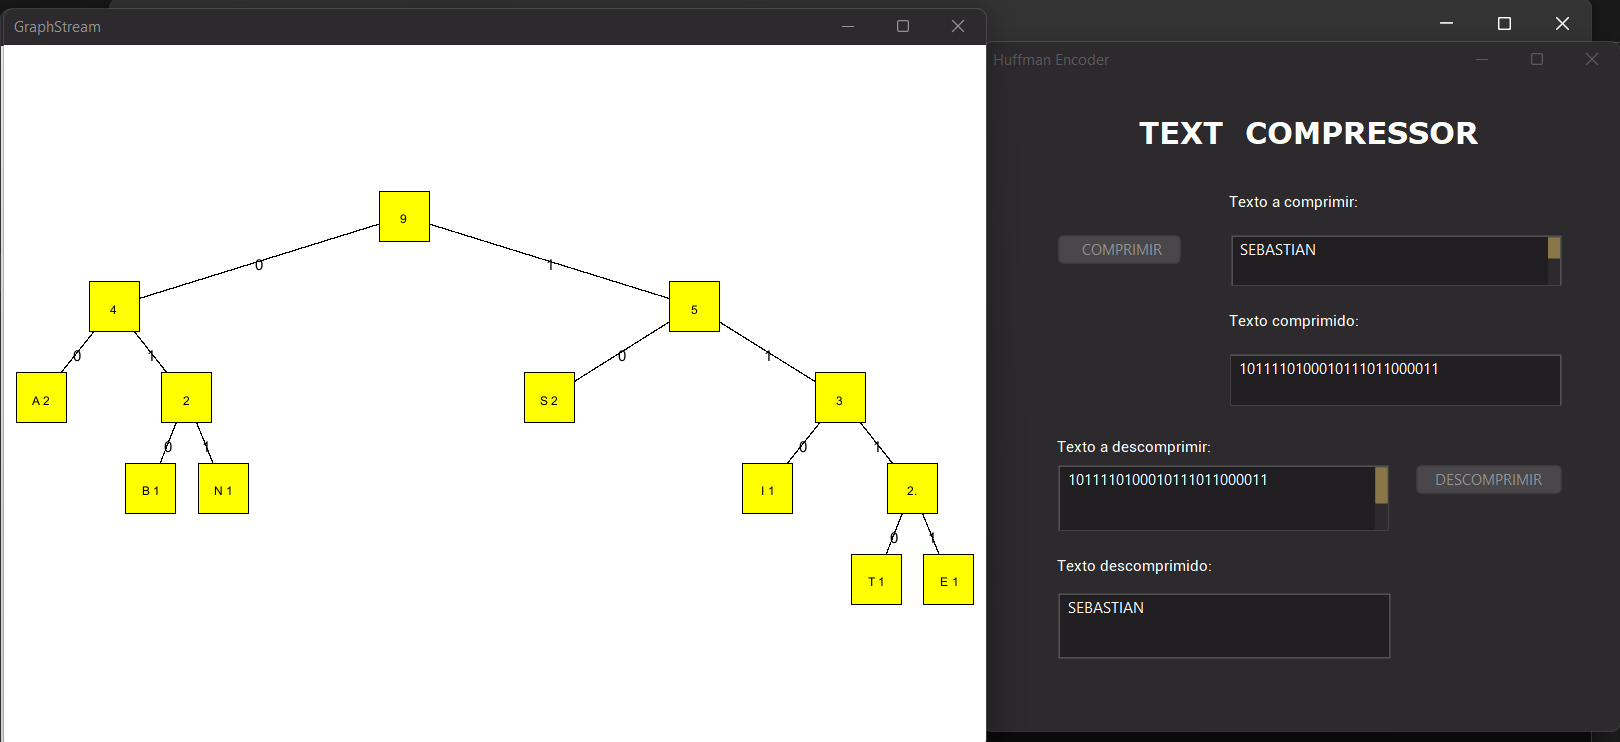
\includegraphics[width=1\textwidth,keepaspectratio]{img/1.png}
	%\includesvg{img/automata.svg}
	%\label{img:mot2}
	%\caption{Product backlog.}
\end{figure}
\begin{itemize}	
	\item EJECUCION 2
\end{itemize}	

\begin{figure}[H]
	\centering
	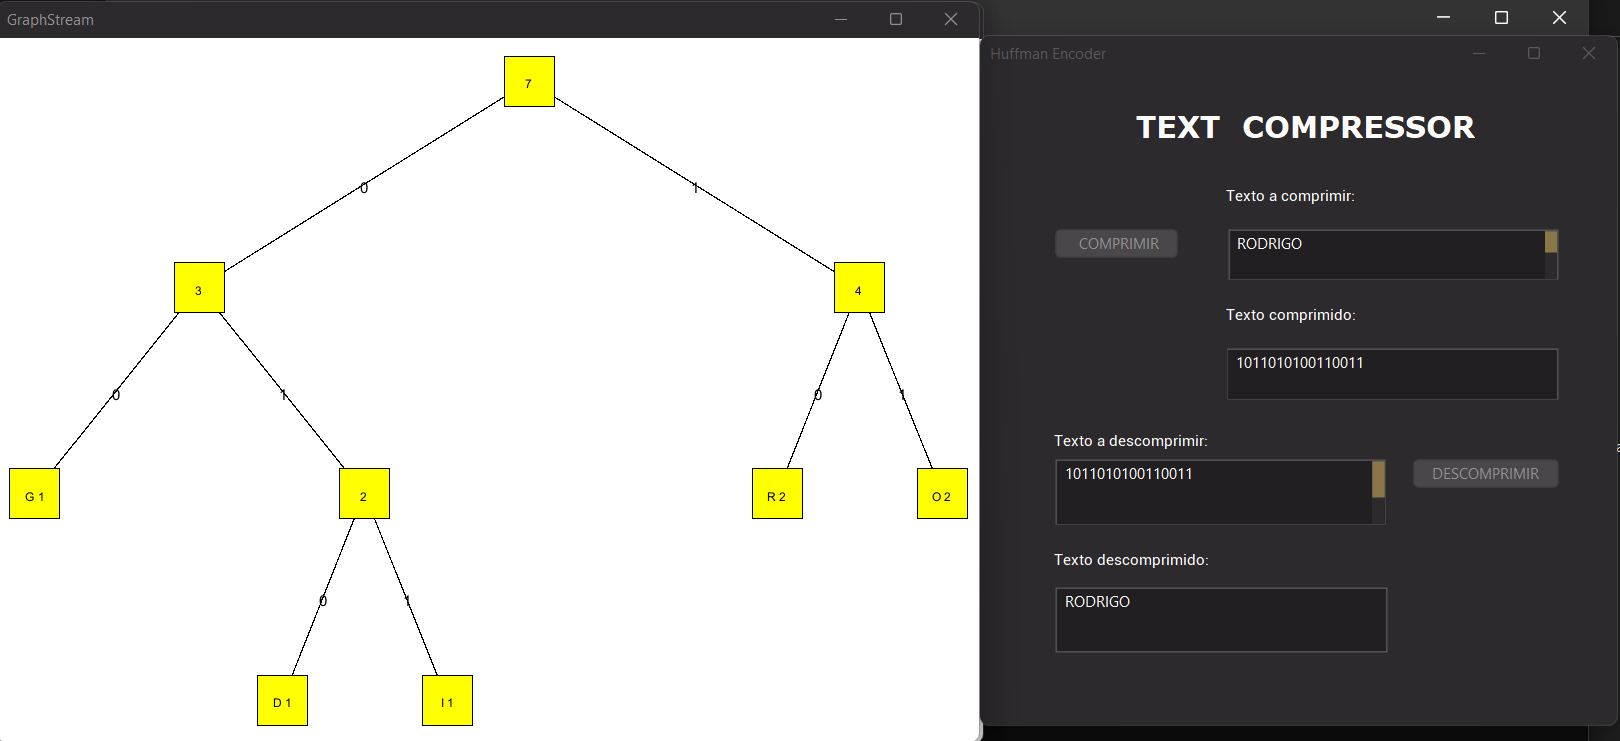
\includegraphics[width=1\textwidth,keepaspectratio]{img/2.png}
	%\includesvg{img/automata.svg}
	%\label{img:mot2}
	%\caption{Product backlog.}
\end{figure}
\begin{itemize}	
	\item EJECUCION 3
\end{itemize}	

\begin{figure}[H]
	\centering
	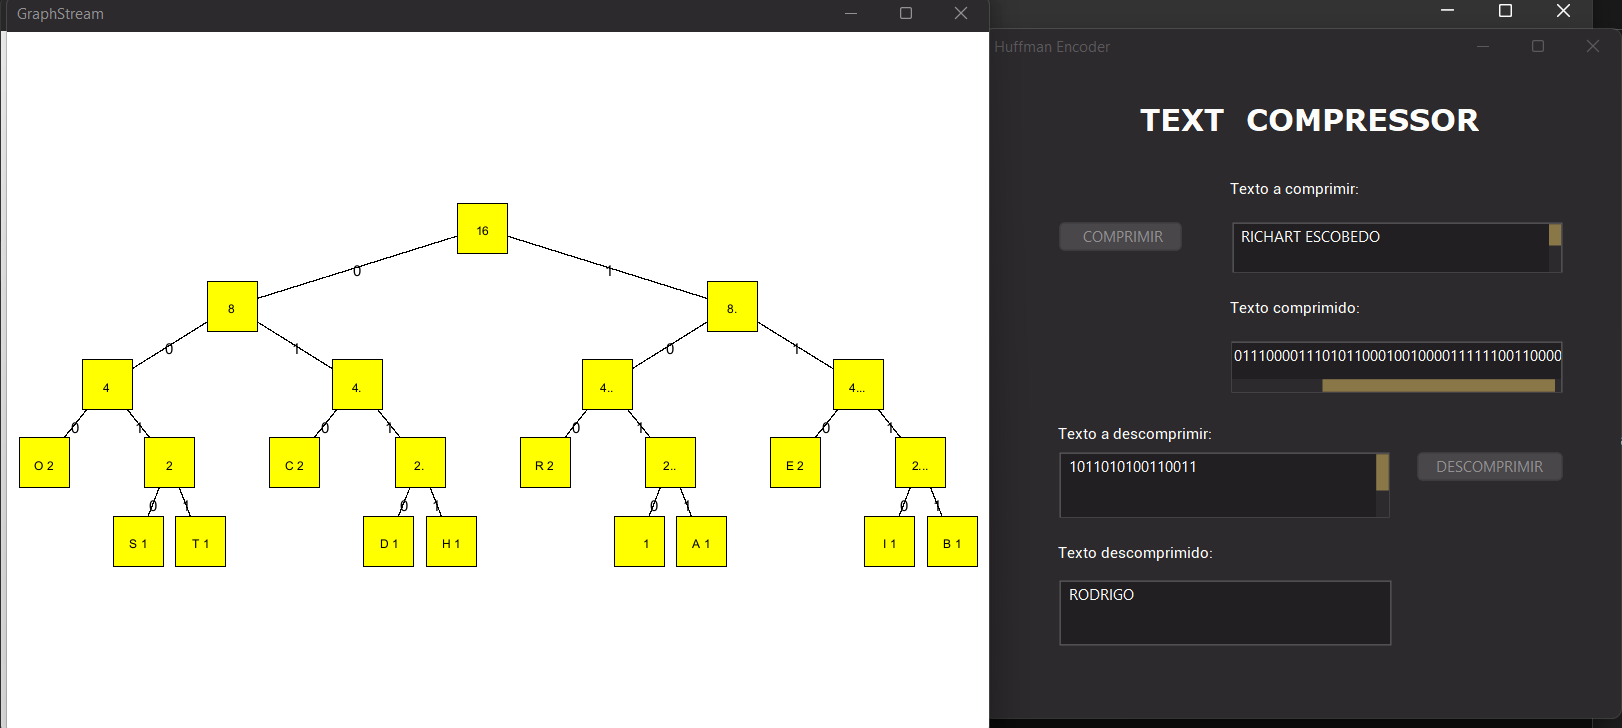
\includegraphics[width=1\textwidth,keepaspectratio]{img/3.png}
	%\includesvg{img/automata.svg}
	%\label{img:mot2}
	%\caption{Product backlog.}
\end{figure}

%%%%%%%%%%%%%%%%%%%%%%%%%%%%%%%%%%%%%%%%%%%%%%%%%%%%%%%%%%%%%%%%%%%%%%%%%%%%%%%%%%


	\subsection{Commits del trabajo}
	\begin{itemize}	
		\item Acá estan algunos de los commits mas importantes en este trabajo:
	\end{itemize}	
	
	\begin{figure}[H]
		\centering
		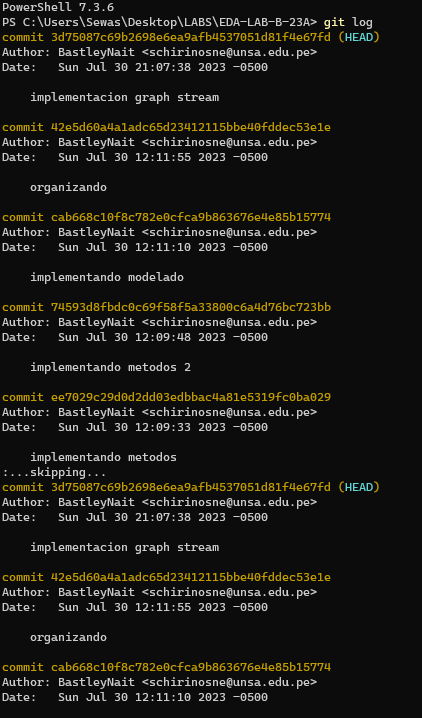
\includegraphics[width=0.7\textwidth,keepaspectratio]{img/Commits.png}
		%\includesvg{img/automata.svg}
		%\label{img:mot2}
		%\caption{Product backlog.}
	\end{figure}


%%%%%%%%%%%%%%%%%%%%%%%%%%%%%%%%%%%%%%%%%%%%%%%%%%%%%%%%%%%%%%%%%%%%%%%%%%%%%%%%%%
\subsection{Instrucciones para la ejecucion}

	\lstinputlisting[language=Bash, caption={EJECUCION.txt},numbers=left,]{src/EJECUCION.txt}	

		
	\subsection{Estructura de laboratorio 08}
	\begin{itemize}	
		\item El contenido que se entrega en este laboratorio es el siguiente:
	\end{itemize}
	
\begin{lstlisting}[style=ascii-tree]
lab08/
|   .gitignore
|	HuffmanTree.java
|	TextCompressor.java
|	Leaf.form
|	NodoHuff.java
\---latex
    |	EDA_lab08.pdf
    |   EDA_lab08.tex
    |
    +---img
    |       Commits.png
    |       logo_abet.png
    |       logo_episunsa.png
    |       logo_unsa.jpg
    |       1.jpg  
    |       2.jpg    
    |		3.jpg
    \---src
		|	HuffmanTree.java
		|	TextCompressor.java
		|	Leaf.form
		|	NodoHuff.java
\end{lstlisting}    


	\section{\textcolor{red}{Rúbricas}}
	
	\subsection{\textcolor{red}{Entregable Informe}}
	\begin{table}[H]
		\caption{Tipo de Informe}
		\setlength{\tabcolsep}{0.5em} % for the horizontal padding
		{\renewcommand{\arraystretch}{1.5}% for the vertical padding
		
		\begin{tabular}{|p{3cm}|p{12cm}|}
			\hline
			\multicolumn{2}{|c|}{\textbf{\textcolor{red}{Informe}}}  \\
			\hline 
			\textbf{\textcolor{red}{Latex}} & \textcolor{blue}{El informe está en formato PDF desde Latex,  con un formato limpio (buena presentación) y facil de leer.}   \\ 
			\hline 
			
			
		\end{tabular}
	}
	\end{table}
	\subsection{\textcolor{red}{Rúbrica para el contenido del Informe y demostración}}
	\begin{itemize}			
		\item El alumno debe marcar o dejar en blanco en celdas de la columna \textbf{Checklist} si cumplio con el ítem correspondiente.
		\item Si un alumno supera la fecha de entrega,  su calificación será sobre la nota mínima aprobada, siempre y cuando cumpla con todos lo items.
		\item El alumno debe autocalificarse en la columna \textbf{Estudiante} de acuerdo a la siguiente tabla:
	
		\begin{table}[ht]
			\caption{Niveles de desempeño}
			\begin{center}
			\begin{tabular}{ccccc}
    			\hline
    			 & \multicolumn{4}{c}{Nivel}\\
    			\cline{1-5}
    			\textbf{Puntos} & Insatisfactorio 25\%& En Proceso 50\% & Satisfactorio 75\% & Sobresaliente 100\%\\
    			\textbf{2.0}&0.5&1.0&1.5&2.0\\
    			\textbf{4.0}&1.0&2.0&3.0&4.0\\
    		\hline
			\end{tabular}
		\end{center}
	\end{table}	
	
	\end{itemize}
	
	\begin{table}[H]
		\caption{Rúbrica para contenido del Informe y demostración}
		\setlength{\tabcolsep}{0.5em} % for the horizontal padding
		{\renewcommand{\arraystretch}{1.5}% for the vertical padding
		%\begin{center}
		\begin{tabular}{|p{2.7cm}|p{7cm}|x{1.3cm}|p{1.2cm}|p{1.5cm}|p{1.1cm}|}
			\hline
    		\multicolumn{2}{|c|}{Contenido y demostración} & Puntos & Checklist & Estudiante & Profesor\\
			\hline
			\textbf{1. GitHub} & Hay enlace URL activo del directorio para el  laboratorio hacia su repositorio GitHub con código fuente terminado y fácil de revisar. &2 &X &2 & \\ 
			\hline
			\textbf{2. Commits} &  Hay capturas de pantalla de los commits más importantes con sus explicaciones detalladas. (El profesor puede preguntar para refrendar calificación). &4 & x&4 & \\ 
			\hline 
			\textbf{3. Código fuente} &  Hay porciones de código fuente importantes con numeración y explicaciones detalladas de sus funciones. &2 &X &2 & \\ 
			\hline 
			\textbf{4. Ejecución} & Se incluyen ejecuciones/pruebas del código fuente  explicadas gradualmente. &2 &X &2 & \\ 
			\hline			
			\textbf{5. Pregunta} & Se responde con completitud a la pregunta formulada en la tarea.  (El profesor puede preguntar para refrendar calificación).  &2 &X &2 & \\ 
			\hline	
			\textbf{6. Fechas} & Las fechas de modificación del código fuente estan dentro de los plazos de fecha de entrega establecidos. &2 &X &2 & \\ 
			\hline 
			\textbf{7. Ortografía} & El documento no muestra errores ortográficos. &2 &X &2 & \\ 
			\hline 
			\textbf{8. Madurez} & El Informe muestra de manera general una evolución de la madurez del código fuente,  explicaciones puntuales pero precisas y un acabado impecable.   (El profesor puede preguntar para refrendar calificación).  &4 &x &4 & \\ 
			\hline
			\multicolumn{2}{|c|}{\textbf{Total}} &20 & &20 & \\ 
			\hline
		\end{tabular}
		%\end{center}
		%\label{tab:multicol}
		}
	\end{table}
	
\clearpage		
\section{Referencias}
\begin{itemize}			
	\item \url{https://www.geeksforgeeks.org/introduction-to-avl-tree/}
	\item \url{https://www.geeksforgeeks.org/insertion-in-an-avl-tree/}
	\item \url{https://www.geeksforgeeks.org/deletion-in-an-avl-tree/}
	\item \url{https://docs.oracle.com/javase/tutorial/java/generics/types.html}
	\item \url{https://algorithmtutor.com/Data-Structures/Tree/AVL-Trees/}

\end{itemize}	

	
%\clearpage
%\bibliographystyle{apalike}
%\bibliographystyle{IEEEtranN}
%\bibliography{bibliography}
			
\end{document}